% --- Configuration ------------------------------------------------------
% add shortcut for github url of this chapter
\def \GITHUB {\GITHUBBASE/01_introduction}
% add the fig folders
\graphicspath{%
{\PATH/\CHAPONE/}%
{\PATH/\CHAPONE/fig1_01/}%
{\PATH/\CHAPONE/fig1_02/}%
{\PATH/\CHAPONE/fig1_03/}%
{\PATH/\CHAPONE/fig1_04/}%
}

% --- Document -----------------------------------------------------------
\chapter{Introduction}
\label{cha:introduction}
%
\firstthought{This document} provides mathematical derivations of the equations that are
implemented in the Sound Field Synthesis Toolbox.\sidenote{The Toolbox is
available at
\href{https://github.com/sfstoolbox/sfs/}{\color{link}https://github.com/sfstoolbox/sfs/}
and was first described in
\cite{Wierstorf2012a}}

We decided to create the Toolbox and this documentation in order to fully allow
for the principle of \emph{reproducible research}\sidenote{\cite[For one of the
pioneers see][]{Donoho2009}} in the research area of \ac{SFS}.
Like other fields that involve signal processing, the study of \ac{SFS}
implies implementing a multitude of algorithms and running numerical simulations
on a computer.
As a consequence, the outcome of the algorithms are easily vulnerable to
implementation errors which cannot completely be
avoided.\sidenote[][]{\cite[Compare][]{Ince2012}}

Functions derived in the theoretical chapter that are implemented in the
toolbox are accompanied by a link to the corresponding function. All figures in
this document have a link in the form of \reproduce{\GITHUBBASE} which is a link to a
folder containing all the data and scripts in order to reproduce the single
figures.

This document is mainly based on the PhD thesis of Hagen
Wierstorf.\autocite{Wierstorf2014} It starts with a small introduction to the
history of spatial sound presentation and presents afterwards the theory of
sound field synthesis, including the derivation of lots of different driving
functions.


%%%%%%%%%%%%%%%%%%%%%%%%%%%%%%%%%%%%%%%%%%%%%%%%%%%%%%%%%%%%%%%%%%%%%%%%%%%%%%%%
\section{Spatial Sound Presentation}

The first ever practical attempt of spatial sound reproduction dates back to
1881, only five years after the invention of the first monaural transducer.
Back then, two parallel telephone channels were used to transmit recorded
music to the homes of the listeners.\autocite{DuMoncel1881a}
The basic idea was the ability to influence the interaural
differences between the two ear signals of the listener. That was achieved by
recording a sound scene with two microphones placed at different positions 
and feeding the recorded signals to the two telephone channels.

Later on the idea advanced to the technique of \emph{binaural presentation} where the basic
principle is to recreate the ear signals at both ears as they would appear in reality.
This can
be achieved by placing two microphones in the ears of the listener for recording and playing the
recorded signals back via headphones afterwards.
Binaural presentation has advanced in the last decades by measuring the
acoustical transmission paths between a source and the ears of a listener, so called
\acp{HRTF}. Afterwards these can be used to create any sound scene as long as
the required \acp{HRTF} are available.
%
\begin{figure}[t]
    \centering
    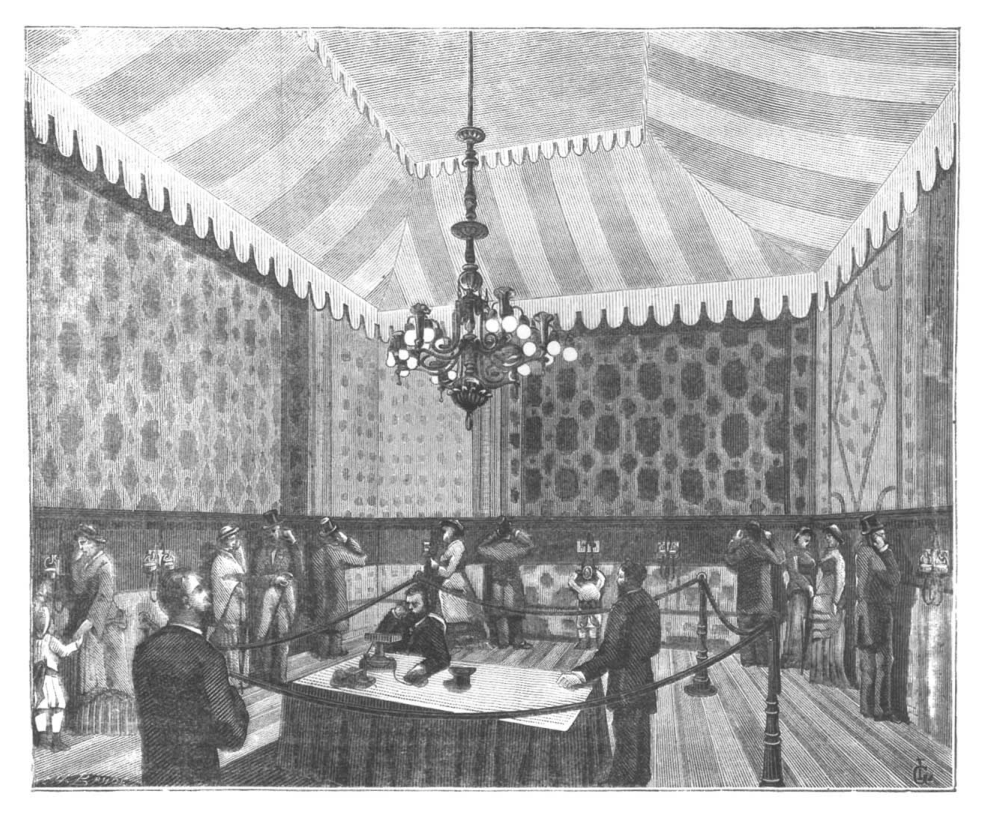
\includegraphics[width=.8\columnwidth]{fig1_01/stereo_telephone}
    \caption{Setup of stereophonic telephones at the exhibition 1881 in
    Paris. Figure from \cite{DuMoncel1881a}
        \reproduce{\GITHUB/fig1_01}
    }
    \label{fig:stereo_telephone}
\end{figure}

Spatial sound presentation via loudspeakers started in the 1930s, the time when
Blumlein invented the stereophonic recording and
reproduction\sidenote[][]{\cite{Blumlein1958}} and Steinberg and Snow discussed the idea of
the acoustical curtain.\autocite{Steinberg1934}
The original idea of the latter was to create a sound field that mimics the real sound
scene. Their practical implementation with two or three loudspeakers was not able
to achieve this. With such low numbers of loudspeakers the sound field is only
controllable at single points in space. This corresponds to the classical
stereophonic setup consisting of a fixed listener position between the two
loudspeakers at a distance of around $2$\,m.
The human head has a diameter of around $20$\,cm and hence only one ear can
be placed at the point where the sound field is as desired. But as Steinberg and
Snow discovered for their acoustic curtain, the spatial perception of the
listener is not disturbed as long as she does not move too far away from a line
on which every point has the same distance to both loudspeakers.
By staying on that line the listener perceives an
auditory event in the center of both loudspeakers, if the same acoustical signal
is played through them. If the amplitude of one of the loudspeakers is changed
the auditory event is moved between the two speakers. The connection of the
amplitude difference between the loudspeakers and the actual position of the
auditory event is empirical and is described by so called panning
laws.\sidenote[][]{\cite{Leakey1959}}
If the listener leaves the central line, the position of the auditory event
will always be located at the position of one of the two loudspeakers. The area in which the
spatial perception of the auditory scene works without considerable impairments
is called the \emph{sweet-spot} of a given loudspeaker setup. It is indicated
by the blue color in Figure\,\ref{fig:stereophony}.
To explain why the spatial perception of the listener is correct at the
sweet-spot although the sound field is not, the theory of \emph{summing
localization} was introduced by Warncke in 1941.\sidenote[][]{\cite[A discussion is
provided in][p.\,204]{Blauert1997}}

In the last years the stereophonic setup was expanded to 5.0 surround
and even larger setups\sidenote[][]{\cite[E.g.][]{Hamasaki2005}} and the panning laws were
formulated in a more general way dealing with setups using multiple
loudspeakers.\sidenote[][]{\cite{Pulkki1997}}
These approaches could not fix the sweet-spot problem, but added a richer
spatial impression because sound is no longer restricted to come from the front.
%
\begin{figure}[t]
    \centering
    \small
    \begin{tikzpicture}
        \draw (-3,0)      node {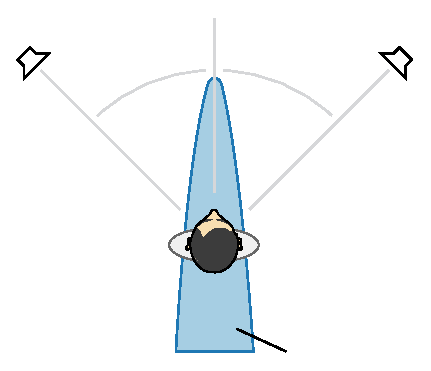
\includegraphics[width=.4\columnwidth]{fig1_02/stereo}};
        \draw (3,0)       node {
\includegraphics[width=.45\columnwidth]{fig1_02/sfs}};
        \draw (-3,3)      node {stereophony};
        \draw (3,3)       node {sound field synthesis};
        \draw (-3.6,0.7)  node {\color{lightgray}\ft $30\degree$};
        \draw (-2.35,0.7) node {\color{lightgray}\ft $30\degree$};
        \draw (-2,-1.93)  node {\ft sweet-spot};
    \end{tikzpicture}
    \caption{Loudspeaker setups for two channel stereophony
    and sound field synthesis. The area marked in blue describes the positions were the
    listener can move to and still perceives the same spatial impression. This
    area is smaller for stereophonic setups and is called the
    sweet-spot. The figure of the stereophony setup is a modified version of
    \cite[][Fig.\,1.1]{Ahrens2012}.
    \reproduce{\GITHUB/fig1_02}}
    \label{fig:stereophony}
\end{figure}

Before 5.0 surround there were other approaches to enhance the spatial impression of
stereophony. From the 1970s onwards quadro\-phony and
Ambisonics\autocite{Gerzon1973} were developed in
order to provide a surround experience with four loudspeakers. The basic idea of
Ambisonics is comparable to nowadays \ac{NFC-HOA} for
a larger number of loudspeakers: to describe an extended sound field by spherical
basis functions that can be synthesized by any spherical or circular loudspeaker
setup. In practice, the restriction of the limited number of loudspeakers has led to the usage
of only two spherical basis functions. The results are
loudspeaker signals that are comparable to the case of panning in
stereophony with the difference of more active
loudspeakers.\autocite[E.g.][]{Frank2013}
If more than four loudspeakers and more than two basis functions
are applied the term is changed to \ac{HOA} to highlight this fact.
For the perceptual side of Ambisonics the sweet-spot problem exists as well.
The explanation of this sweet-spot is only partly covered by the
theory of summing localization, because that theory is not well investigated for
several sound sources coming from all directions. This provoked a high number of
different optimizations of the loudspeaker signals by the Ambisonics community.


All of the methods described so far are able to provide a
convincing spatial impression at a specific listener position within the
loudspeaker setup. That means none of them can handle an equally good spatial
impression for a bigger audience.

In the late 1980s the old idea of Steinberg and Snow to reproduce a
complete sound field came to new life due to the fact that now arrangements of
more than 100 loudspeakers became possible.\autocite{Berkhout1988}
This high number of loudspeakers is needed: for controlling an extended
sound field up to $20$\,kHz, loudspeaker spacings under $1$\,cm
are required. Small distances like that are not possible in practice. Nonetheless,
the experience has shown that even with larger distances reasonable sound field
approximations are possible. Some of them provide equal spatial impression in the
whole listening area, as indicated by the blue color in Figure\,\ref{fig:stereophony}.
Methods trying to achieve this goal are summarized under the term \acf{SFS}.
This document focusses on the two \ac{SFS} techniques \ac{WFS} and \ac{NFC-HOA}
that are explained in detail in the next chapter.


%%%%%%%%%%%%%%%%%%%%%%%%%%%%%%%%%%%%%%%%%%%%%%%%%%%%%%%%%%%%%%%%%%%%%%%%%%%%%%%%
\section{Mathematical Definitions}
\label{sec:mathematical_definitions}
%
\begin{figure}
    \centering
    \small
    % GNUPLOT: LaTeX picture with Postscript
\begingroup
  \makeatletter
  \providecommand\color[2][]{%
    \GenericError{(gnuplot) \space\space\space\@spaces}{%
      Package color not loaded in conjunction with
      terminal option `colourtext'%
    }{See the gnuplot documentation for explanation.%
    }{Either use 'blacktext' in gnuplot or load the package
      color.sty in LaTeX.}%
    \renewcommand\color[2][]{}%
  }%
  \providecommand\includegraphics[2][]{%
    \GenericError{(gnuplot) \space\space\space\@spaces}{%
      Package graphicx or graphics not loaded%
    }{See the gnuplot documentation for explanation.%
    }{The gnuplot epslatex terminal needs graphicx.sty or graphics.sty.}%
    \renewcommand\includegraphics[2][]{}%
  }%
  \providecommand\rotatebox[2]{#2}%
  \@ifundefined{ifGPcolor}{%
    \newif\ifGPcolor
    \GPcolortrue
  }{}%
  \@ifundefined{ifGPblacktext}{%
    \newif\ifGPblacktext
    \GPblacktextfalse
  }{}%
  % define a \g@addto@macro without @ in the name:
  \let\gplgaddtomacro\g@addto@macro
  % define empty templates for all commands taking text:
  \gdef\gplbacktext{}%
  \gdef\gplfronttext{}%
  \makeatother
  \ifGPblacktext
    % no textcolor at all
    \def\colorrgb#1{}%
    \def\colorgray#1{}%
  \else
    % gray or color?
    \ifGPcolor
      \def\colorrgb#1{\color[rgb]{#1}}%
      \def\colorgray#1{\color[gray]{#1}}%
      \expandafter\def\csname LTw\endcsname{\color{white}}%
      \expandafter\def\csname LTb\endcsname{\color{black}}%
      \expandafter\def\csname LTa\endcsname{\color{black}}%
      \expandafter\def\csname LT0\endcsname{\color[rgb]{1,0,0}}%
      \expandafter\def\csname LT1\endcsname{\color[rgb]{0,1,0}}%
      \expandafter\def\csname LT2\endcsname{\color[rgb]{0,0,1}}%
      \expandafter\def\csname LT3\endcsname{\color[rgb]{1,0,1}}%
      \expandafter\def\csname LT4\endcsname{\color[rgb]{0,1,1}}%
      \expandafter\def\csname LT5\endcsname{\color[rgb]{1,1,0}}%
      \expandafter\def\csname LT6\endcsname{\color[rgb]{0,0,0}}%
      \expandafter\def\csname LT7\endcsname{\color[rgb]{1,0.3,0}}%
      \expandafter\def\csname LT8\endcsname{\color[rgb]{0.5,0.5,0.5}}%
    \else
      % gray
      \def\colorrgb#1{\color{black}}%
      \def\colorgray#1{\color[gray]{#1}}%
      \expandafter\def\csname LTw\endcsname{\color{white}}%
      \expandafter\def\csname LTb\endcsname{\color{black}}%
      \expandafter\def\csname LTa\endcsname{\color{black}}%
      \expandafter\def\csname LT0\endcsname{\color{black}}%
      \expandafter\def\csname LT1\endcsname{\color{black}}%
      \expandafter\def\csname LT2\endcsname{\color{black}}%
      \expandafter\def\csname LT3\endcsname{\color{black}}%
      \expandafter\def\csname LT4\endcsname{\color{black}}%
      \expandafter\def\csname LT5\endcsname{\color{black}}%
      \expandafter\def\csname LT6\endcsname{\color{black}}%
      \expandafter\def\csname LT7\endcsname{\color{black}}%
      \expandafter\def\csname LT8\endcsname{\color{black}}%
    \fi
  \fi
  \setlength{\unitlength}{0.0500bp}%
  \begin{picture}(4534.00,2834.00)%
    \gplgaddtomacro\gplbacktext{%
      \csname LTb\endcsname%
      \put(254,1125){\makebox(0,0){\strut{}$z$}}%
      \colorrgb{0.65,0.81,0.89}%
      \put(1320,687){\makebox(0,0)[l]{\strut{}$\phi$}}%
      \put(1318,955){\makebox(0,0)[l]{\strut{}$\theta$}}%
      \colorrgb{0.12,0.47,0.71}%
      \put(2629,2070){\makebox(0,0)[l]{\strut{}\vec{x}}}%
    }%
    \gplgaddtomacro\gplfronttext{%
      \csname LTb\endcsname%
      \put(2166,240){\makebox(0,0){\strut{}$x$}}%
      \put(761,1449){\makebox(0,0){\strut{}$y$}}%
      \put(254,1125){\makebox(0,0){\strut{}$z$}}%
    }%
    \gplbacktext
    \put(0,0){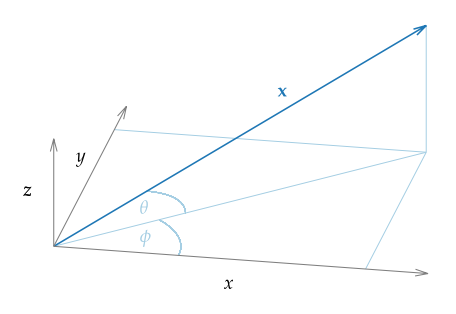
\includegraphics{coordinate_system}}%
    \gplfronttext
  \end{picture}%
\endgroup

    \caption{Coordinate system used in this thesis. The vector $\vec{x}$ can also
    be described by its length, its azimuth angle $\phi$, and its elevation
    $\theta$.
    \reproduce{\GITHUB/fig1_03}}
    \label{fig:coordinate_system}
\end{figure}
%
\paragraph{Coordinate system}
Figure\,\ref{fig:coordinate_system} shows the coordinate system that is used in
the following chapters. A vector $\vec{x}$ can be described by its position
$(x,y,z)$ in space or by its length, azimuth angle $\phi \in [0,2\PI[$,
and elevation $\theta \in \left[-\frac{\PI}{2},\frac{\PI}{2}\right]$.
The azimuth is measured counterclockwise and elevation is positive
for positive $z$-values.


%----%----%----%----%----%----%----%----%----%----%----%----%----%----%----%----
\paragraph{Fourier transformation}
Let $s$ be an absolute integrable function, $t,\omega$ real numbers, then the
temporal Fourier transform is defined as\autocite{Bracewell2000}
%
\begin{equation}
    S(\omega) = \FT{s(t)} = \int^{\infty}_{-\infty} s(t) \E^{-\I\omega t}
    \; \D{t}
    \qp
    \tag{\#az9}
    \label{eq:ft}
\end{equation}

In the same way the inverse temporal Fourier transform is defined as
%
\begin{equation}
    s(t) = \IFT{S(\omega)} = \frac{1}{2\PI} \int^{\infty}_{-\infty} S(\omega)
    \E^{\I\omega t} \; \D\omega
    \qp
    \tag{\#2zg}
    \label{eq:ift}
\end{equation}
